% The generic preamble
\documentclass[10pt,letterpaper,fleqn,titlepage]{report}

% Define packages to use
\usepackage{natbib}
\usepackage[dvips]{graphicx,color}
\usepackage{amsmath,amssymb}
\usepackage{bm}
\usepackage{caption}
\usepackage{xr}
\usepackage{ifthen}
\usepackage[dvipdfm,colorlinks,linkcolor=blue,citecolor=blue,urlcolor=blue]{hyperref}
\usepackage{fancybox}
\usepackage{textcomp}
\usepackage{fancyhdr}
\usepackage{titlesec}
\usepackage{multirow}
\usepackage{alltt}
\usepackage{svn}
\usepackage{longtable}

\titleformat{\chapter}[frame]
  {\normalfont}
  {\filright\slshape\Huge\enspace\thechapter\enspace}
  {8pt}
  {\normalfont\Huge\filcenter\slshape\sffamily} 

\titleformat{\section}[hang]
  {\normalfont}
  {\filright\sffamily\bfseries\Large\thesection}
  {5pt}
  {\normalfont\Large\filright\sffamily\bfseries}[\vspace{2pt}\titlerule]

\titleformat{\subsection}[hang]
  {\normalfont}
  {\filright\slshape\sffamily\large\thesubsection}
  {5pt}
  {\normalfont\large\filright\slshape\sffamily} 
  
% Redefine default page
\setlength{\textheight}{9.0in}  % 1" above and below
\setlength{\textwidth}{6.75in}   % 0.5" left and right
\setlength{\oddsidemargin}{-0.25in}
\setlength{\topmargin}{0.0pt}
\setlength{\headsep}{16.0pt}

% Redefine default paragraph
\setlength{\parindent}{0pt}
\setlength{\parskip}{1.5ex plus 0.5ex minus 0.2ex}

% Define caption width and default fonts
\setlength{\captionmargin}{0.5in}
\renewcommand{\captionfont}{\sffamily}
\renewcommand{\captionlabelfont}{\bfseries\sffamily}

% Defined commands
\newcommand{\superscript}[1]{\ensuremath{^\textrm{#1}}}
\newcommand{\subscript}[1]{\ensuremath{_\textrm{#1}}}
\newcommand{\invcm}{\textrm{cm\superscript{-1}}}
\newcommand{\micron}{\ensuremath{\mu\textrm{m}}}
\newcommand{\textbfm}[1]{\boldmath\ensuremath{#1}\unboldmath}
\newcommand{\water}{\textrm{H\subscript{2}O}}
\newcommand{\carbondioxide}{\textrm{CO\subscript{2}}}
\newcommand{\ozone}{\textrm{O\subscript{3}}}
\newcommand{\methane}{\textrm{CH\subscript{4}}}
\newcommand{\nitrousoxide}{\textrm{N\subscript{2}O}}
\newcommand{\carbonmonoxide}{\textrm{CO}}

% Define how equations are numbered
\numberwithin{equation}{chapter}
\numberwithin{figure}{chapter}
\numberwithin{table}{chapter}

% Space/nudging commands
\newcommand{\rb}[1]{\raisebox{1.5ex}[0pt]{#1}}

%Redefine the enumerate environment to decrease the item spacing.
\let\oldenumerate=\enumerate
\let\endoldenumerate=\endenumerate
\renewenvironment{enumerate}{%
  \begin{oldenumerate}%
    \setlength{\itemsep}{0ex}%
  }%
  {%
  \end{oldenumerate}%
  }

% Define a command for title page author email footnote
\newcommand{\email}[1]
{%
  \renewcommand{\thefootnote}{\alph{footnote}}%
  \footnote{#1}
  \renewcommand{\thefootnote}{\arabic{footnote}}
}

% Redefine the maketitle macro
\makeatletter
\renewcommand{\maketitle}
{%
  \thispagestyle{empty}
  \vspace*{1in}
  \begin{center}%
     \sffamily
     {\huge\bfseries Joint Center for Satellite Data Assimilation\par}%
  \end{center}
  \begin{flushleft}%
     \sffamily
     \vspace*{0.5in}
     {\Large\bfseries CRTM: \@title\par}%
     \medskip
     {\large\@author\par}%
     \medskip
     {\large\@date\par}%
     \bigskip\hrule\vspace*{2pc}%
  \end{flushleft}%
  \newpage
  \setcounter{footnote}{0}
}
\makeatother


% Define a command for a DRAFT watermark
\usepackage{eso-pic}
\newcommand{\draftwatermark}
{
  \AddToShipoutPicture{%
    \definecolor{lightgray}{gray}{.85}
    \setlength{\unitlength}{1in}
    \put(2.5,3.5){%
      \rotatebox{45}{%
        \resizebox{4in}{1in}{%
          \textsf{\textcolor{lightgray}{DRAFT}}
        }
      }
    }
  }
}


% Define included documents
%\includeonly{}

% Title info
\title{Implementation of FASTEM-4 in the CRTM}
\author{Paul van Delst\footnote{paul.vandelst@noaa.gov}\\JCSDA/EMC/IMSG\\[0.25in]
        David N. Groff\footnote{david.groff@noaa.gov}\\JCSDA/EMC/IMSG.}
\date{April, 2011}
\docnumber{1}

%-------------------------------------------------------------------------------
%                            Ze document begins...
%-------------------------------------------------------------------------------
\begin{document}
\maketitle

%\draftwatermark

\section{Radiometric Impact of Implementing FASTEM-4 into the CRTM}
The radiometric impact of implementing FASTEM-4 for any particular CRTM simulation depends on the channel central frequency, salinity, sea-surface temperature, surface wind speed and the angle between the wind direction and the sensor azimuth angle.  For a standard tropical atmosphere we performed CRTM simulations using FASTEM-4 and the MWSSEM that was used in CRTM release 2.0.2 for NOAA-19 AMSUA, NOAA-19 MHS, F16 SSMIS and Aqua AMSRE to assess how the magnitude of the radiometric impact depends on these inputs.  CRTM simulations for release 2.0.2 were based on the 'Low Frequency' model for channel frequencies less than 20 GHz and FASTEM1 for channel frequencies greater than 20 GHz. 

\subsection{Dependance on Channel Frequency}
The channel central frequency determines the sensitivity to the surface and accounts for the most significant variability in the impact on CRTM simulations.  For example as shown in figure \ref{fig:AMSUA_Wind_Speed_Impact} the magnitude of the impact on simulations for AMSUA NOAA-19 can vary from channel to channel by more than 5K.  With the exception of AMSRE Aqua channels 1-4 the CRTM simulations using FASTEM-4 are colder for all the surface conditions we considered.  For AMSRE channels 1-4 the CRTM simulations using FASTEM-4 can be 5K larger as shown in figure \ref{fig:AMSRE_Wind_Speed_Impact}.  Note that for AMSRE channels 1-6 the low frequency emissivity model was used.

\begin{figure}[htp]
  \centering
  \includegraphics[scale=0.75]{graphics/AMSUA_Wind_Speed_BT.eps}
  \caption{The radiometric impact of implementing FASTEM-4 on AMSUA NOAA-19 simulations as a function of wind speed.}
  \label{fig:AMSUA_Wind_Speed_Impact}
\end{figure}

\newpage

\begin{figure}[htp]
  \centering
  \includegraphics[scale=0.75]{graphics/AMSRE_Wind_Speed_BT.eps}
  \caption{The radiometric impact of implementing FASTEM-4 on AMSRE Aqua simulations as a function of wind speed.}
  \label{fig:AMSRE_Wind_Speed_Impact}
\end{figure}

%\newpage

\subsection{Dependence on Wind Speed}
The impact on CRTM simulations for microwave channels sensitive to the surface is most dependant on wind speed.  Figure \ref{fig:AMSUA_Wind_Speed_Impact} shows that the magnitude of the impact at wind speeds approaching 15 m/s are on the order of 2K larger than at wind speeds less than 4 m/s.  This result is corroborated by Figure \ref{fig:AMSUA_Background_Impact} which shows scatter plots of impact as brightness temperature differences for AMSUA MetOP-A using global NCEP background data from February 2, 2009 and August 1, 2009 as input.  The scatter plots for both days illustrate that the impact on MetOP-A AMSUA simulations increases with wind speed.

\begin{figure}[htp]
  \centering
  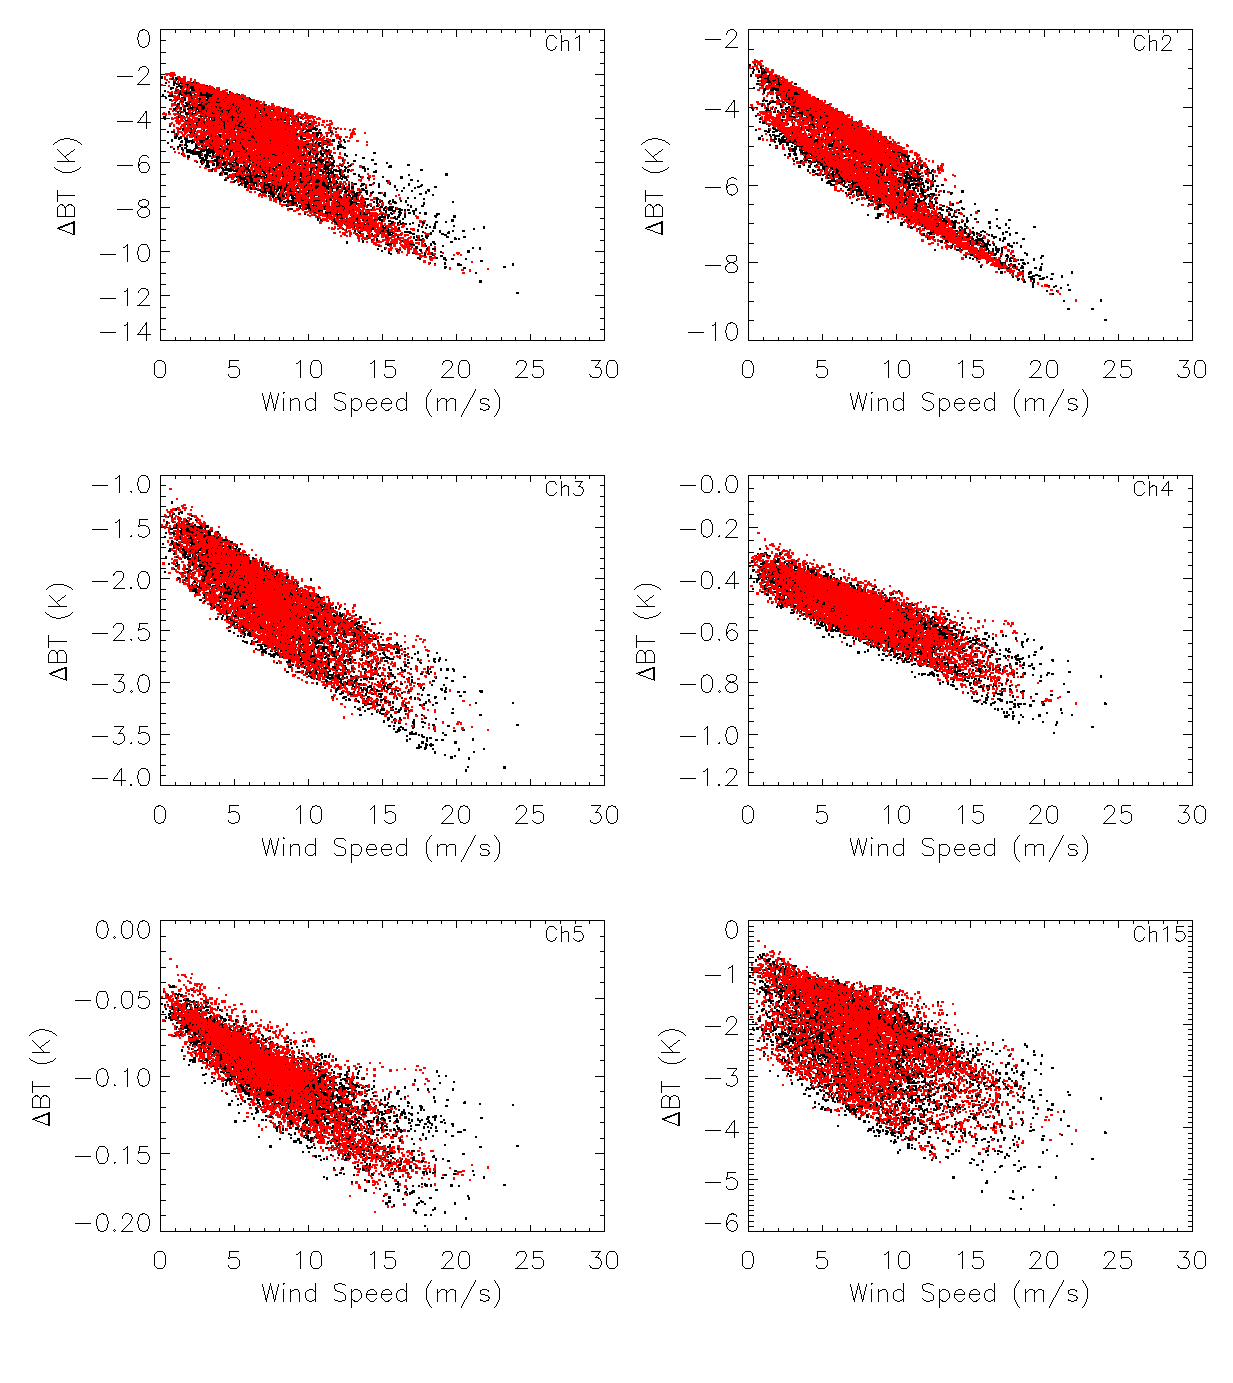
\includegraphics[scale=0.75]{graphics/emissD_windS_f.eps}
  \caption{The radiometric impact on MetOP-A AMSUA simulations as a function of wind speed using global NCEP background data from February 2, 2009 and August 1, 2009 as input .}
  \label{fig:AMSUA_Background_Impact}
\end{figure}

\newpage

\subsection{Dependence on Salinity}
For AMSUA and MHS surface channels the impact decreases with increasing salinity as shown in figures \ref{fig:AMSUA_Salinity_Impact} and \ref{fig:MHS_Salinity_Impact}.  

\begin{figure}[htp]
  \centering
  \includegraphics[scale=0.75]{graphics/AMSUA_Salinity_BT.eps}
  \caption{The radiometric impact of implementing FASTEM-4 on AMSUA NOAA-19 simulations as a function of salinity.}
  \label{fig:AMSUA_Salinity_Impact}
\end{figure}

\begin{figure}[htp]
  \centering
  \includegraphics[scale=0.75]{graphics/MHS_Salinity_BT.eps}
  \caption{The radiometric impact of implementing FASTEM-4 on MHS NOAA-19 simulations as a function of salinity.}
  \label{fig:MHS_Salinity_Impact}
\end{figure}

\newpage

\subsection{Dependence on the Angle Between the Sensor Azimuth and Wind Direction} 
The impact can vary significantly as a function of the angle between the sensor azimuth and wind direction.  The impact increases with the perpendicularity of the sensor azimuth to the wind direction.  When the sensor azimuths are perpedicular to the CRTM default wind direction (North) the magnitude of the brightness temperature differences are nearly 1K larger than those at sensor azimuths parallel or opposite to the wind direction as shown in figure \ref{fig:AMSUA_Sensor_Azimuth_Impact}.  

\begin{figure}[htp]
  \centering
  \includegraphics[scale=0.75]{graphics/AMSUA_Sensor_Azimuth_BT.eps}
  \caption{The radiometric impact of implementing FASTEM-4 as a function of the angle between the wind direction and sensor azimuth.}
  \label{fig:AMSUA_Sensor_Azimuth_Impact}
\end{figure} 

% The references section
%=======================
%\clearpage
%\bibliographystyle{plainnat}
%\bibliography{bibliography}
%\begin{thebibliography}{99}
%  \bibitem{ref:tag1} reference1
%  \bibitem{ref:tag2} reference2
%\end{thebibliography}

% The appendices section
%=======================
%\begin{appendix}
%\end{appendix}

\end{document}
